\documentclass{standalone}
\usepackage{tikz}
\usetikzlibrary{patterns, positioning}

\begin{document}
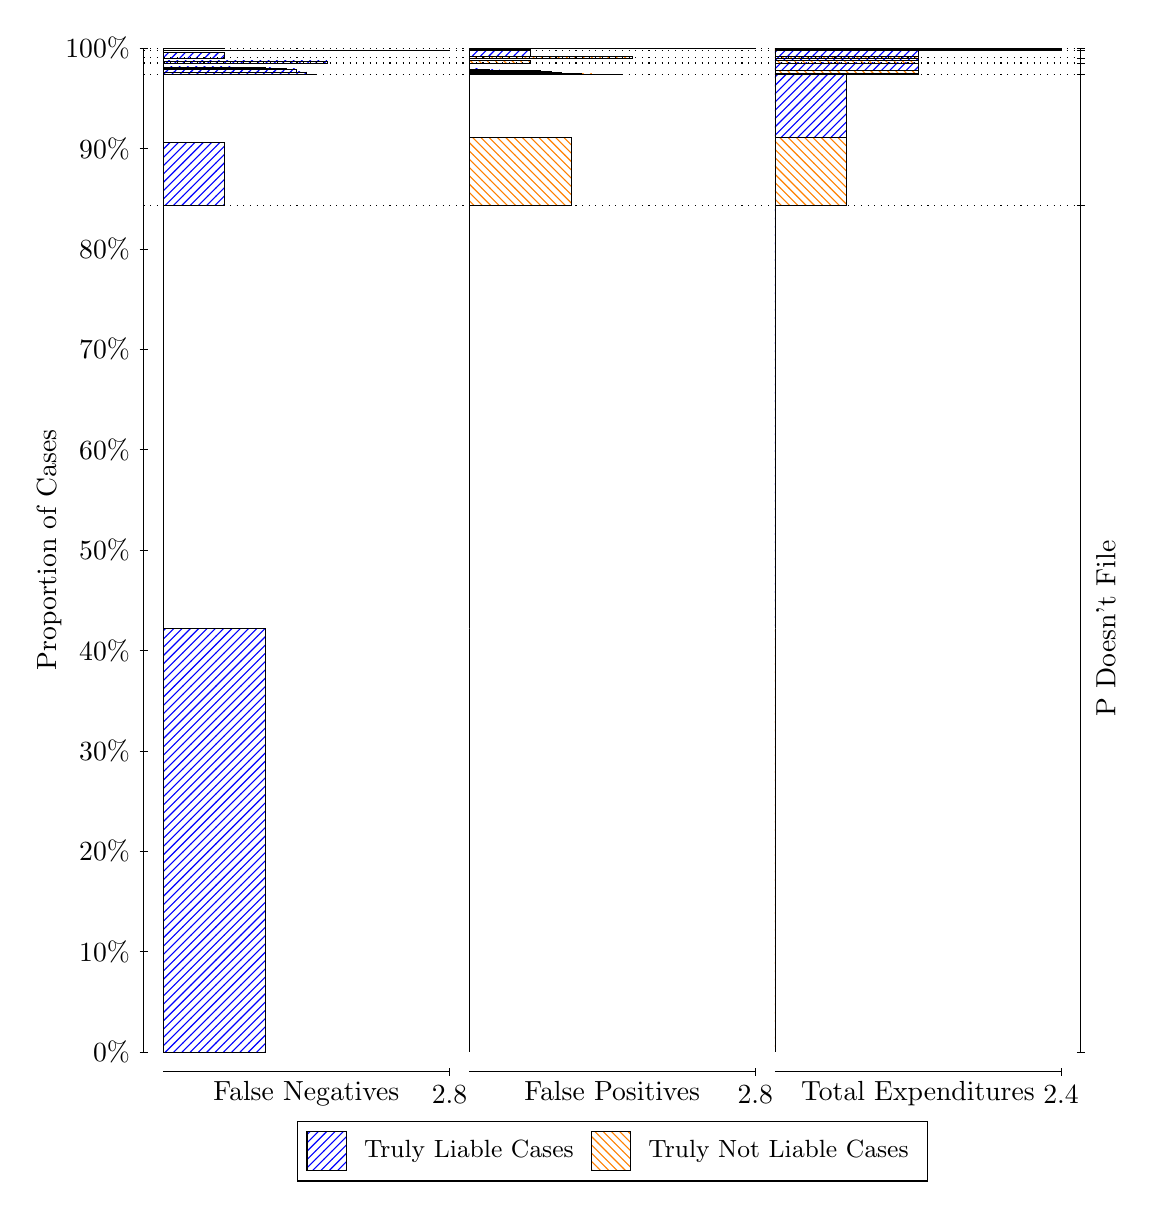
\begin{tikzpicture}
\draw[black, very thin] (1.5,1.75) -- (1.5,14.5);
\node[rotate=90, anchor=center] at (0.3, 8.125) {Proportion of Cases};
\draw[black, very thin] (1.45,1.75) -- (1.55,1.75);
\node[anchor=east] at (1.45, 1.75) {0\%};
\draw[black, very thin] (1.45,3.025) -- (1.55,3.025);
\node[anchor=east] at (1.45, 3.025) {10\%};
\draw[black, very thin] (1.45,4.3) -- (1.55,4.3);
\node[anchor=east] at (1.45, 4.3) {20\%};
\draw[black, very thin] (1.45,5.575) -- (1.55,5.575);
\node[anchor=east] at (1.45, 5.575) {30\%};
\draw[black, very thin] (1.45,6.85) -- (1.55,6.85);
\node[anchor=east] at (1.45, 6.85) {40\%};
\draw[black, very thin] (1.45,8.125) -- (1.55,8.125);
\node[anchor=east] at (1.45, 8.125) {50\%};
\draw[black, very thin] (1.45,9.4) -- (1.55,9.4);
\node[anchor=east] at (1.45, 9.4) {60\%};
\draw[black, very thin] (1.45,10.675) -- (1.55,10.675);
\node[anchor=east] at (1.45, 10.675) {70\%};
\draw[black, very thin] (1.45,11.95) -- (1.55,11.95);
\node[anchor=east] at (1.45, 11.95) {80\%};
\draw[black, very thin] (1.45,13.225) -- (1.55,13.225);
\node[anchor=east] at (1.45, 13.225) {90\%};
\draw[black, very thin] (1.45,14.5) -- (1.55,14.5);
\node[anchor=east] at (1.45, 14.5) {100\%};

\draw[black, very thin] (13.4,1.75) -- (13.4,14.5);
\draw[black, very thin] (13.35,1.75) -- (13.45,1.75);
\node[anchor=west] at (13.35, 1.75) {};
\draw[black, very thin] (13.35,12.505) -- (13.45,12.505);
\node[anchor=west] at (13.35, 12.505) {};
\draw[black, very thin] (13.35,14.164) -- (13.45,14.164);
\node[anchor=west] at (13.35, 14.164) {};
\draw[black, very thin] (13.35,14.31) -- (13.45,14.31);
\node[anchor=west] at (13.35, 14.31) {};
\draw[black, very thin] (13.35,14.375) -- (13.45,14.375);
\node[anchor=west] at (13.35, 14.375) {};
\draw[black, very thin] (13.35,14.466) -- (13.45,14.466);
\node[anchor=west] at (13.35, 14.466) {};
\draw[black, very thin] (13.35,14.493) -- (13.45,14.493);
\node[anchor=west] at (13.35, 14.493) {};
\draw[black, very thin] (13.35,14.5) -- (13.45,14.5);
\node[anchor=west] at (13.35, 14.5) {};

\draw[black, very thin, pattern color=blue, pattern=north east lines] (1.75,1.75) rectangle (3.0476,7.1273);
\draw[black, very thin, pattern color=orange, pattern=north west lines] (1.75,7.1273) rectangle (1.75,12.505);
\draw[black, very thin, pattern color=blue, pattern=north east lines] (1.75,12.505) rectangle (2.5286,13.299);
\draw[black, very thin, pattern color=orange, pattern=north west lines] (1.75,13.299) rectangle (1.75,14.164);
\draw[black, very thin, pattern color=blue, pattern=north east lines] (1.75,14.164) rectangle (3.6964,14.168);
\draw[black, very thin, pattern color=blue, pattern=north east lines] (1.75,14.168) rectangle (3.5667,14.197);
\draw[black, very thin, pattern color=blue, pattern=north east lines] (1.75,14.197) rectangle (3.4369,14.235);
\draw[black, very thin, pattern color=blue, pattern=north east lines] (1.75,14.235) rectangle (3.3071,14.24);
\draw[black, very thin, pattern color=blue, pattern=north east lines] (1.75,14.24) rectangle (3.1774,14.247);
\draw[black, very thin, pattern color=blue, pattern=north east lines] (1.75,14.247) rectangle (3.0476,14.252);
\draw[black, very thin, pattern color=blue, pattern=north east lines] (1.75,14.252) rectangle (2.9179,14.257);
\draw[black, very thin, pattern color=blue, pattern=north east lines] (1.75,14.257) rectangle (2.7881,14.259);
\draw[black, very thin, pattern color=blue, pattern=north east lines] (1.75,14.259) rectangle (2.6583,14.261);
\draw[black, very thin, pattern color=orange, pattern=north west lines] (1.75,14.261) rectangle (1.75,14.31);
\draw[black, very thin, pattern color=blue, pattern=north east lines] (1.75,14.31) rectangle (3.8262,14.338);
\draw[black, very thin, pattern color=orange, pattern=north west lines] (1.75,14.338) rectangle (1.75,14.375);
\draw[black, very thin, pattern color=blue, pattern=north east lines] (1.75,14.375) rectangle (2.5286,14.446);
\draw[black, very thin, pattern color=orange, pattern=north west lines] (1.75,14.446) rectangle (1.75,14.466);
\draw[black, very thin, pattern color=blue, pattern=north east lines] (1.75,14.466) rectangle (5.3833,14.469);
\draw[black, very thin, pattern color=orange, pattern=north west lines] (1.75,14.469) rectangle (1.75,14.493);
\draw[black, very thin, pattern color=blue, pattern=north east lines] (1.75,14.493) rectangle (2.5286,14.497);
\draw[black, very thin, pattern color=orange, pattern=north west lines] (1.75,14.497) rectangle (1.75,14.5);
\draw[black, very thin, pattern color=orange, pattern=north west lines] (5.6333,1.75) rectangle (5.6333,7.1274);
\draw[black, very thin, pattern color=blue, pattern=north east lines] (5.6333,7.1274) rectangle (5.6333,12.505);
\draw[black, very thin, pattern color=orange, pattern=north west lines] (5.6333,12.505) rectangle (6.931,13.37);
\draw[black, very thin, pattern color=blue, pattern=north east lines] (5.6333,13.37) rectangle (5.6333,14.164);
\draw[black, very thin, pattern color=orange, pattern=north west lines] (5.6333,14.164) rectangle (7.5798,14.166);
\draw[black, very thin, pattern color=orange, pattern=north west lines] (5.6333,14.166) rectangle (7.45,14.167);
\draw[black, very thin, pattern color=orange, pattern=north west lines] (5.6333,14.167) rectangle (7.3202,14.169);
\draw[black, very thin, pattern color=orange, pattern=north west lines] (5.6333,14.169) rectangle (7.1905,14.172);
\draw[black, very thin, pattern color=orange, pattern=north west lines] (5.6333,14.172) rectangle (7.0607,14.176);
\draw[black, very thin, pattern color=orange, pattern=north west lines] (5.6333,14.176) rectangle (6.931,14.179);
\draw[black, very thin, pattern color=orange, pattern=north west lines] (5.6333,14.179) rectangle (6.8012,14.192);
\draw[black, very thin, pattern color=orange, pattern=north west lines] (5.6333,14.192) rectangle (6.6714,14.201);
\draw[black, very thin, pattern color=orange, pattern=north west lines] (5.6333,14.201) rectangle (6.5417,14.213);
\draw[black, very thin, pattern color=blue, pattern=north east lines] (5.6333,14.213) rectangle (6.2821,14.215);
\draw[black, very thin, pattern color=blue, pattern=north east lines] (5.6333,14.215) rectangle (6.1524,14.218);
\draw[black, very thin, pattern color=blue, pattern=north east lines] (5.6333,14.218) rectangle (6.0226,14.222);
\draw[black, very thin, pattern color=blue, pattern=north east lines] (5.6333,14.222) rectangle (5.8929,14.227);
\draw[black, very thin, pattern color=blue, pattern=north east lines] (5.6333,14.227) rectangle (5.7631,14.234);
\draw[black, very thin, pattern color=blue, pattern=north east lines] (5.6333,14.234) rectangle (5.6333,14.31);
\draw[black, very thin, pattern color=orange, pattern=north west lines] (5.6333,14.31) rectangle (6.4119,14.346);
\draw[black, very thin, pattern color=blue, pattern=north east lines] (5.6333,14.346) rectangle (5.6333,14.375);
\draw[black, very thin, pattern color=orange, pattern=north west lines] (5.6333,14.375) rectangle (7.7095,14.395);
\draw[black, very thin, pattern color=blue, pattern=north east lines] (5.6333,14.395) rectangle (6.4119,14.466);
\draw[black, very thin, pattern color=orange, pattern=north west lines] (5.6333,14.466) rectangle (6.4119,14.49);
\draw[black, very thin, pattern color=blue, pattern=north east lines] (5.6333,14.49) rectangle (5.6333,14.493);
\draw[black, very thin, pattern color=orange, pattern=north west lines] (5.6333,14.493) rectangle (9.2667,14.496);
\draw[black, very thin, pattern color=blue, pattern=north east lines] (5.6333,14.496) rectangle (7.969,14.5);
\draw[black, very thin, pattern color=orange, pattern=north west lines] (9.5167,1.75) rectangle (9.5167,7.1274);
\draw[black, very thin, pattern color=blue, pattern=north east lines] (9.5167,7.1274) rectangle (9.5167,12.505);
\draw[black, very thin, pattern color=orange, pattern=north west lines] (9.5167,12.505) rectangle (10.425,13.37);
\draw[black, very thin, pattern color=blue, pattern=north east lines] (9.5167,13.37) rectangle (10.425,14.164);
\draw[black, very thin, pattern color=orange, pattern=north west lines] (9.5167,14.164) rectangle (11.333,14.169);
\draw[black, very thin, pattern color=blue, pattern=north east lines] (9.5167,14.169) rectangle (11.333,14.176);
\draw[black, very thin, pattern color=orange, pattern=north west lines] (9.5167,14.176) rectangle (11.333,14.217);
\draw[black, very thin, pattern color=blue, pattern=north east lines] (9.5167,14.217) rectangle (11.333,14.3);
\draw[black, very thin, pattern color=orange, pattern=north west lines] (9.5167,14.3) rectangle (11.333,14.303);
\draw[black, very thin, pattern color=blue, pattern=north east lines] (9.5167,14.303) rectangle (11.333,14.31);
\draw[black, very thin, pattern color=orange, pattern=north west lines] (9.5167,14.31) rectangle (11.333,14.346);
\draw[black, very thin, pattern color=blue, pattern=north east lines] (9.5167,14.346) rectangle (11.333,14.375);
\draw[black, very thin, pattern color=orange, pattern=north west lines] (9.5167,14.375) rectangle (11.333,14.395);
\draw[black, very thin, pattern color=blue, pattern=north east lines] (9.5167,14.395) rectangle (11.333,14.466);
\draw[black, very thin, pattern color=orange, pattern=north west lines] (9.5167,14.466) rectangle (13.15,14.49);
\draw[black, very thin, pattern color=blue, pattern=north east lines] (9.5167,14.49) rectangle (13.15,14.493);
\draw[black, very thin, pattern color=orange, pattern=north west lines] (9.5167,14.493) rectangle (13.15,14.496);
\draw[black, very thin, pattern color=blue, pattern=north east lines] (9.5167,14.496) rectangle (13.15,14.5);
\draw[black, dotted] (1.5,12.505) -- (13.4,12.505);
\draw[black, dotted] (1.5,14.164) -- (13.4,14.164);
\draw[black, dotted] (1.5,14.31) -- (13.4,14.31);
\draw[black, dotted] (1.5,14.375) -- (13.4,14.375);
\draw[black, dotted] (1.5,14.466) -- (13.4,14.466);
\draw[black, dotted] (1.5,14.493) -- (13.4,14.493);
\draw[black, very thin] (1.75,1.5) -- (5.3833,1.5);
\node[anchor=north] at (3.5667, 1.5) {False Negatives};
\draw[black, very thin] (5.3833,1.45) -- (5.3833,1.55);
\node[anchor=north] at (5.3833, 1.45) {2.8};

\draw[black, very thin] (5.6333,1.5) -- (9.2667,1.5);
\node[anchor=north] at (7.45, 1.5) {False Positives};
\draw[black, very thin] (9.2667,1.45) -- (9.2667,1.55);
\node[anchor=north] at (9.2667, 1.45) {2.8};

\draw[black, very thin] (9.5167,1.5) -- (13.15,1.5);
\node[anchor=north] at (11.333, 1.5) {Total Expenditures};
\draw[black, very thin] (13.15,1.45) -- (13.15,1.55);
\node[anchor=north] at (13.15, 1.45) {2.4};

\node[black, centered, rotate=90] at (13.72, 7.1274) {P Doesn't File};







\draw (7.449999999999999,1.5) node[draw=none] (baseCoordinate) {};
\begin{scope}[align=center]
        \matrix[scale=0.5, draw=black, below=0.5cm of baseCoordinate, nodes={draw}, column sep=0.1cm]{
            \node[rectangle, draw, minimum width=0.5cm, minimum height=0.5cm, pattern=north east lines, pattern color=blue] {}; &
            \node[draw=none, font=\small] (B) {Truly Liable Cases}; &
            \node[rectangle, draw, minimum width=0.5cm, minimum height=0.5cm, pattern=north west lines, pattern color=orange] {}; &
            \node[draw=none, font=\small] (B) {Truly Not Liable Cases}; \\
            };
\end{scope}

\end{tikzpicture}
\end{document}